\chapter{Topology and Knotting in Soft Matter Systems}

\section{Introduction: Kelvin's vortex atom}
The original, and perhaps most familiar, example of a knotted field is the smoke ring. Easily made by cutting a circular hole in a rectangular box, then replacing the opposite side entirely with a sheet of rubber, ``a blow on this flexible side causes a circular vortex ring to shoot out from the hole on the other side'' \citep{Kelvin}. In 1867, exactly this demonstration was shown to Lord Kelvin by Peter Guthrie Tait. What is generated is a tightly circulating tube of air, closed into a ring, which propagates stably across the room, rebounding elastically from walls and even other vortex rings (of course to see the ring one first needs to fill the box with smoke, perhaps using dry ice or ``a small quantity of muriatic acid'' \citep{Kelvin}). At the time, the microscopic nature of atoms was still under debate, and the stability of the rings, a consquence of Helmholtz's laws of vortex motion in an ideal fluid \citep{Helmholtz} (translated into English by Tait), coupled with their elasticity and capacity for internal vibration \citep{KelvinMasters, KelvinAMS} prompted Kelvin to suggest that ``Helmholtz's rings are the only true atoms". Suitably knotted and linked, these rings might form the microscopic basis of all matter \citep{Kelvin,Thomson}.

Kelvin's ``vortex atom'' rapidly encountered difficulties in its mathematical content, its falsifiability, and a lack of contempory experimental support \citep{KelvinMasters}. However its content, summarised as ``\textit{Physics = Geometry}'' in Ref. \citep{KelvinAMS}, was compelling (perhaps slightly dangerously so) and apparently motivated Tait, in ``consideration of the forms of knots by Sir W. Thomson's (Lord Kelvin) Theory of Vortex Atoms'', to construct the first systematic tables of knots in 1876--1885 (Figure \ref{fig:History}) \citep{Tait}. These articles, alongside a ``very remarkable essay by Listing ... and an acute remark made by Gauss ... with some comments on it by Clerk-Maxwell'' \citep{Tait}form the initial studies in  what is now the mathematical field of Knot Theory \cite{Lickorish}. Maxwell himself, although not an active contributor to vortex atom theory, had a clear interest in the ideas, encouraging Tait and Kelvin to ``prosper and disentangle your formulae in proportion as you entangle your worbles'' (Figure \ref{fig:History}) \citep{MaxwellTaitLetter}. Indeed the ``comments'' referred to by Tait are in fact Maxwell's rederivation of Gauss's Linking number, as presented in his \textit{Treatise on Electricity and Magnetsim} in 1873, about which we will have much more to say in \ref{ch2}. 

Despite forming the starting point for modern knot theory, the knotted structures above are quite different to those found in your shoelaces, or in the world of art and design outside the physics department\footnote{or so I am told.}. Rather than a single knotted curve, we have a continuous fluid in whose structure the knot is embedded, and from which dynamical properties of the knot (its motion, stability, a spectrum of vibrational modes etc.) may be derived. Such structures are referred to as \emph{knotted fields}, of which the vortex atom may be considered a prototype. This disconnect is reflected in Tait's work, which mentions Kelvin's Vortex Atoms briefly as motivation, but focuses in substance on ``\emph{the investigation of the essentially different modes of joining points in a plane}'' \citep{Tait}. As knot theory developed, its initial connections to hydrodynamics and electromagnetism --- in other words, the importance of the physical field in which the knot was embedded ---  were further abandoned. We also note that despite the wonderful knot tables produced by Tait (figure \ref{fig:History}) and the reliance of vortex atom theory on knotted and linked vortices, there is no mention above of any experimental evidence on vortices tied in nontrivial knots. 

\section{Modern knotted fields}

The first experimental construction of a nontrivial knotted field came 140 years after the first theoretical investigations of their dynamics, from the Irvine lab in 2013 \cite{Kleckner2013}.

\begin{figure}[tb]
\centering
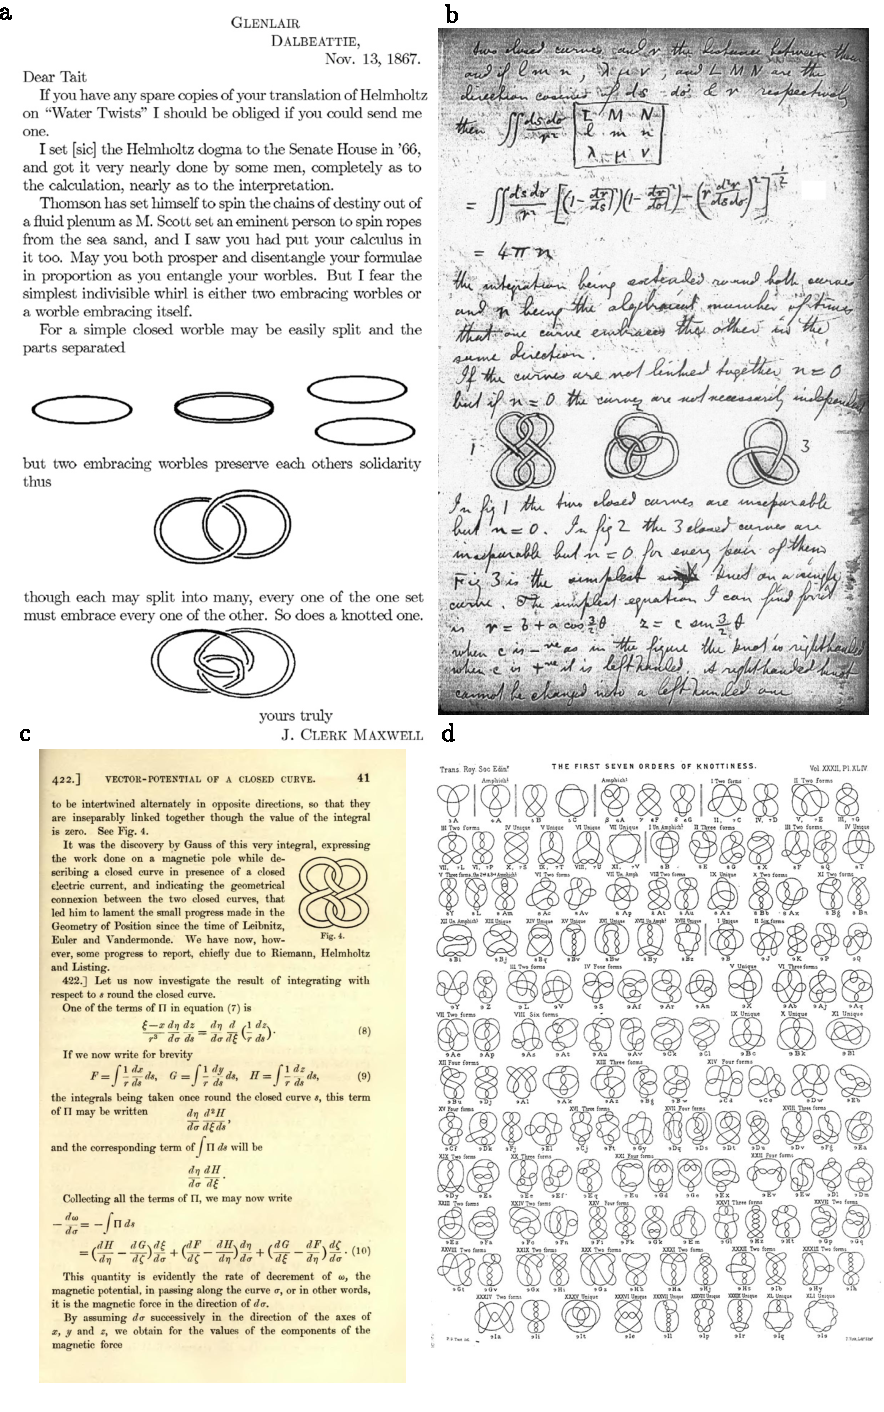
\includegraphics[width=0.99\linewidth]{\IntroductionFigures/History.pdf}
\caption{hi }
\label{fig:History}
\end{figure}
